\documentclass[12pt,a4paper,oneside]{book}
\usepackage[a4paper,%
            left=35mm,right=20mm,top=20mm,bottom=20mm]{geometry}
\usepackage{titlesec} 
\usepackage{fancyhdr}
\usepackage[utf8]{inputenc} 
\usepackage{graphicx}
\usepackage{booktabs} % for much better looking tables
\usepackage{array} % for better arrays (eg matrices) in maths
\usepackage{paralist} % very flexible & customisable lists (eg. enumerate/itemize, etc.)
\usepackage{verbatim} % adds environment for commenting out blocks of text & for better verbatim
\usepackage{subfig} % make it possible to include more than one captioned figure/table in a single 
\usepackage[toc,page]{appendix}
\usepackage{pdfpages}
\usepackage{listings}
\usepackage{color}
\usepackage{graphicx}
\usepackage{subfig}
\usepackage{setspace}
\onehalfspacing
\usepackage{helvet}
\usepackage{mathtools}
\usepackage{float}

%Hyperlinks set to no colours/black
\usepackage{hyperref}
\hypersetup{
    colorlinks=false,
    linkcolor=black,
    filecolor=black,      
    urlcolor=black,
}

\renewcommand{\familydefault}{\sfdefault}

\definecolor{dkgreen}{rgb}{0,0.6,0}

%header and footer settings
\pagestyle{fancyplain}
\fancyhf{}
\renewcommand{\headrulewidth}{0.5pt}
\renewcommand{\footrulewidth}{0.5pt}
\setlength{\headheight}{15pt}
\fancyhead[L]{Adam Blance - 40161070}
\fancyhead[R]{ SOC10101 Honours Project}
\fancyfoot[L]{}
\fancyfoot[C]{\thepage}



%set better section layout
\makeatletter
\renewcommand\subsection{\@startsection {subsection}{1}{2mm} % name, level, indent
                               {3pt plus 2pt minus 1pt} % before skip
                               {3pt plus 0pt} % after skip
                               {\normalfont\bfseries}}
\makeatother
\makeatletter
\renewcommand\section{\@startsection {section}{1}{0mm} % name, level, indent
                               {4pt plus 2pt minus 1pt} % before skip
                               {4pt plus 0pt} % after skip
                               {\bfseries}}
\makeatother


%this starts the document
\begin{document}

\frontmatter

%you can import other documents into your main one, these layout the Title and Declarations on its own page.
%you might need to change these to \ if your on Microsoft Windows.
\newcommand{\HRule}{\rule{\linewidth}{0.5mm}}

\begin{titlepage}
	\begin{center}

	\HRule \\[0.4cm]
    	{\Large \bfseries Evaluation of Procedaully Generatated Escort Mission Maps\par}
	\vspace{0.2cm}
	\HRule \\[1.5cm]

	
    	\vspace{3cm}
	\begin{minipage}{0.4\textwidth}
	\begin{center} \large
        \emph{}\\
        	Adam Blance - 40161070
				
   	 \end{center}
    	\end{minipage}
	
	\vspace{2cm}
    	\begin{minipage}{1\textwidth}
    	\begin{center} \large
        
		Submitted in partial fulfilment of \\
		the requirements of Edinburgh Napier University \\
		for the Degree of \\
        	BSc (Hons) Games Development
    	\end{center}
    	\end{minipage}

    	\vfill

    	% Bottom of the page
	\begin{minipage}{1\textwidth}
    	\begin{center} \large
		School of Computing
    	\end{center}
    	\end{minipage}
	
	\vspace{1cm}
    	{\large \today}


	\end{center}
\end{titlepage}
%{\large Submitted in partial fulfilment of the requirements of Edinburgh Napier University for the Degree of }

\section*{Authorship Declaration}
\vspace{0.5cm}
\begin{flushleft}
I, Adam Blance, confirm that this dissertation and the work presented in it are my own achievement.\newline

Where I have consulted the published work of others this is always clearly attributed;\newline

Where I have quoted from the work of others the source is always given. With the exception of such quotations this dissertation is entirely my own work;\newline

I have acknowledged all main sources of help; \newline

If my research follows on from previous work or is part of a larger collaborative research project I have made clear exactly what was done by others and what I have contributed myself;\newline

I have read and understand the penalties associated with Academic Misconduct.\newline

I also confirm that I have obtained informed consent from all people I have involved in the work in this dissertation following the School's ethical guidelines.\newline
\end{flushleft}

\begin{flushleft} \large
\emph{Signed:} \\
\end{flushleft}

\vspace{.5cm}

\begin{flushleft} \large
\emph{Date:} \\
\end{flushleft}

\vspace{.5cm}

\begin{flushleft} \large
\emph{Matriculation no: }  \\
\end{flushleft}
\pagebreak

\section*{Data Protection Declaration}
\vspace{0.5cm}
\begin{flushleft}
Under the 1998 Data Protection Act, The University cannot disclose your grade to an unauthorised person. However, other students benefit from studying dissertations that have their grades attached. \newline

\vspace{0.5cm}

Please sign your name below one of the options below to state your preference.\newline
\vspace{0.5cm}

The University may make this dissertation, with indicative grade, available to others.\newline
\vspace{3cm}


The University may make this dissertation available to others, but the grade may not be disclosed.\newline
\vspace{3cm}


The University may not make this dissertation available to others.\newline
\end{flushleft}


\pagebreak

\section*{Abstract}
Being able to evaluate certain types of maps can be a very useful tool for game developers of first person shooters. These games can be extremely popular.With the one of largest still boasting a player base of over 30 million a year after the game was released \cite{OverwatchPopularity}. This means that company who could quickly evaluate and release their games could beat out competitors, with the most successful of these likely securing a higher profit margin.
\vspace{5mm} 
\newline
 This dissertation will document the research, implementation and evaluation of an attempt to successfully automate the evaluation process of the release co-operative first person shooter maps and an attempt to procedurally generate these maps was made. We aim to identify what makes a good map and what factors effect the success of these maps.
 \vspace{5mm} 
 \newline
 We look at a variety of games that are currently on the market and have a large player bases along with the maps that are considered the most popular within them. We investigate the similar projects like this and identify the several techniques that maybe suitable for generating a map that can be used to successfully pass the algorithm.
  \vspace{5mm} 
 \newline
 A detailed analysis on these techniques is provided. Also included is the outlining of the process of creating the noise that was generated adhering to the evaluation algorithm and the aspects that are used including Dijkstra's algorithm and binomial distribution. We also discuss the creation of the survey that will be used to test the successfulness of the algorithm and discuss the metrics which will be recorded. 
  \vspace{5mm} 
 \newline 
 The implementation provides a detailed description of the creation process of the evaluation algorithm. A description is provided on the creation of the procedural generated map that was also created. The challenges that were encountered during these tasks are also highlighted.
  \vspace{5mm} 
 \newline 
Analysing the results we were able to draw a number of conclusions; we found that the procedural map generation could successfully pass as professionally made escort mission maps. We also proved that the evaluation algorithm could produce an evaluation of similar calibre to a user review.
\tableofcontents 

\listoftables

\listoffigures

\newpage
\section*{Acknowledgements}
I would like to thank my supervisor, Dr Kevin Chalmers, for all his constant support, thorough out my time in university and I am incredibly grateful for all the times he has listened to and helped with all my concerns and problems.  
 \vspace{5mm} 
\newline 
I would also like to thank my second marker, Dr Gregory Leplatre for his  encouragement,support, and helpful advice that he has given during my time in university.
 \vspace{5mm} 
\newline 
I am also greatly  thankful for all my course mates and my family who have helped me out so much during this year and I greatly valued all the time we have spent together. 
 \vspace{5mm} 
\newline 
Finally I would like to thank the School of Computing for giving me the facilities needed to create this dissertation and give me the knowledge that will help me for the rest of my life.
\newpage

\mainmatter

%INTRO
\chapter{Introduction}
From the beginning of the project the objective has been to develop a mathematical equation to evaluate escort mission maps. Then to procedurally generate maps that can successfully follow the evaluation technique created. The dissertation produced underneath documents the work that was involved in achieving this.
\vspace{5mm} 
\newline
\section{Motivation}
With video games being one of the largest markets in the world right now, gaming companies must be developing and releasing their games as quickly as possible. If there is any conceivable way for them speed up releasing their games, they should take these approaches.
\vspace{5mm} 
\newline  
One of the biggest genres of games currently is team based shooters. With one of the larger games in the genre being Overwatch with currently over 35 million players worldwide.\cite{Overt} This genre of game has a very different development cycle to other games relying on continual updates adding new maps and characters to keep players interested and continually playing. To release new maps and characters on a regular basis can be difficult especially if the game has a large competitive scene because the new feature \vspace{5mm} must be fully tested before released.
\newline  
With testing new features in games becoming the most time consuming part of the development cycle, companies must look into other ways to streamline the testing of games. In this project one of the possible ways to decrease the time taken to test maps is explored. If companies can use a mathematical formula to test the fairness of maps, rather than the more conventional user based testing which can take up to several weeks, would allow for companies to produce more content in a quicker time frame, generating a greater profit and allowing for better content to be produced in the future. 
\vspace{5mm} 
\newline
\section{Aims and Objectives}
There are two main aims of the project, the first is to create, implement and evaluate an algorithm that assesses escort mission maps once this has been complete, the next aim is to plan and develop a piece of software that can successfully follow the algorithm produced. The objectives below have been selected in order to accomplish these aims.
\begin{itemize}
	\item Research relevant topics and papers.
	\item Create or use an existing framework that can be used to develop the map.
	\item Design an algorithm taking into account size, path of the payload and fairness. 
	\item Develop a programme that can procedurally generate escort mission maps.	
\end{itemize}
\vspace{5mm} 
\section{Scope}
\subsection{Deliverable}
The items to be delivered from this project are: An algorithm that can evaluate any escort mission map and inform the user of the strengths and weakness of the map; A C++ program that can procedurally generate maps that can be tested by the algorithm; the results and analysis of the surveys that examine the credibility of the evaluation algorithm.  
\subsection{Boundaries and Constraints}
When testing a map there are a large amount variables to be evaluated, as time is one of the limiting factors in this project, it was decided that 3 major factors would be tested. They are:
\begin{itemize}
	\item The size of the map.
	\item The quality of the object that will be escorted (payload) path.
	\item The overall balance\textbackslash fairness of the map 	
\end{itemize}
\vspace{5mm} 
\section{Chapter Outlines}
\begin{itemize}
	\item Background - Discusses the research made into the topic.
	\item Methodology – States the methods used throughout the implementation process.
	\item Implementation - Details specific techniques and choices that were made during the Implementation phase.
	\item Results – Displays the results from the tests carried out.
	\item Conclusion – Summarises results that were collected , assess the successfulness of the data gathered and discusses future work.	
\end{itemize}

%BACKGROUND
\chapter{Background}
In this section, an investigation into escort mission maps and how to evaluate them is presented. Requirements and challenges are presented, and in particular video game maps are examined. Procedural generation one of the main factors of this project is also examined in depth. Finally path-finding and other evaluating techniques is presented, focusing on how to evaluate maps in video games. 
\vspace{5mm} 
\newline
\section{Co-operative First Person Shooters}
Th with one of the first major titles being Quake in 1996 and other notable series including Call of Duty, Battlefield and Halo, with the objective of the game usually being to get the most eliminations. 
\vspace{5mm} 
\newline
A subsection of this genre is the co-operative first person shooter. This type of game heavily relies on teamwork, with games being won by holding onto an objective or pushing a payload. These games are enjoyable to a wide player base, usually offering a variety of play styles or different characters to use. This attracts a wide player base which translates to a large amount of revenue streams for the company that produced these games; including E-Sports, merchandises and potential Spin-off games. This include Blizzards co-op game Overwatch hitting peak viewer-ship with 441,000 viewers on its English stream during its first day \cite{LukeChristou}
\subsection{Escort Missions}
An escort mission is a game-mode in cooperative first person shooter such as Overwatch and Loadout. In this mode there are two teams, the attacking and the defending team. The two teams have different aims in order to win. The attacking team attempts to escort the payload across the map to an objective while the defending team tries to stop them. It is difficult to pin down the first game to have escort missions. One of the more notable was in 2007 with Team Fortress 2. While it was not originally included in the game it was added in the first free update. It is important to note that the original Team Fortress had a game mode called Escort but this has many differences with its sequel, such as the payload being a controllable player and there being three teams. Other games that use this game mode include Global Agenda and Wolfenstein: Enemy Territory.    
\vspace{5mm} 
\newline
\section{Maps}
In video games, maps are the term used to describe the area that the player can move around in. Different games will have different types of maps depending on how the developer wants the player to play the game. For instance an RPG like Skyrim or The Witcher will usually have a large map for the player to explore the world and find their own path, while other faster paced first person shooters like the Call of Duty franchise might rely on a more linear map to construct the most enjoyable experience for their players. It is very important for a programmer to constantly be planning and evaluating the map they are creating as this will directly affect how enjoyable the game they created is.
\vspace{5mm} 
\newline
\section{Escort Mission Maps}
Escort mission maps are the play areas that escort missions are performed in. Between each game these maps can vary greatly so for this project, the definition of an escort mission map must be stated. The maps must have an attacking and defending spawn area. This is the place where the teams start at the beginning of the match and will return too whenever they die. The map must also have an unobstructed route that runs between the spawns, which the payload will be moved through. This route will be generated using path-finding algorithm which is discussed below.
\vspace{5mm} 
\newline 
\section{Procedural Generation in Video Games}
Typically when a game is being made their is a time constraint as the company will not have the resources to spend a large period of time developing their game. Usually data will have to be created manually which can be very time consuming, however several short-cuts can be made.
\vspace{5mm} 
\newline
Procedural generation is a technique that can be used  to generate data algorithmically and can be used to greatly reduce the time taken for the creation of large systems within the game. This can lead to a less predictable game and can also reduce the memory size of the game. It has been used in several large title such as; an entire galaxy in No Man's Sky and was used in the weapon generation in the very popular Borderlands series.  
\subsection{Procedurally Generated Maps}
It is very common in gaming to use procedural generation, as it allows companies to take short-cuts when creating the game, and allows them to focus on more time consuming aspects of the game such as; graphics and game-play. Procedural generation has been used in many video games for a variety of things. This includes weapon generation in the Borderlands series and Spore which uses procedural generation to create animals and evolve them. However the most common use of procedural generation is to create the map. This has been used in many notable games including, Minecraft , No Man’s Sky and Dwarf Fortress. These create huge worlds for the player to roam around in and can allow the map to go on forever. Procedural generation will be used in the project on a much smaller scale then most games to generate the map but it will be used in conjunction with other techniques such as path-finding.  
\vspace{5mm} 
\newline
\section{Path-Finding}
Many games today have implemented an advanced artificial intelligence for a variety of reasons, an important aspect of this path-finding. This is used for a variety of reasons such as enemy’s movement and being used for troop movements in real time strategy games. Path-finding is way for a computer to calculate the shortest route between two points. It does this by searching a graph by starting at one vertex and evaluating the neighbouring nodes. The most common of the path-finding algorithms is Dijkstra's algorithm.	
\subsection{Dijkstra’s Algorithm}
Published by Edsger W. Dijkstra in 1959, Dijkstra’s algorithm is a way to calculate the shortest path between nodes on a graph. Solving the single-source shortest path problem. Nodes on a graph can represent either a 2-dimensional grid or points in a 3-D space. The most common example of a real life application of Dijkstra’s algorithm is being used in geographical maps to plot the fastest route between two cities, where each city is a node and the roads are associated with a weight. 
\vspace{2mm} 
\newline
\begin{figure}[H]
	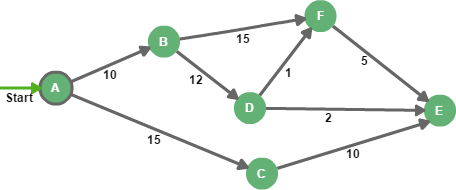
\includegraphics[width=\linewidth]{images/Dijsk.png}
	\caption{A weighted graph of connected nodes}
\end{figure}
The algorithm works by initially marking the distance from the starting point to every other vertex on the graph. All nodes are then set to unvisited and are stored  by priority within a queue. The next step would be to compare all unvisited neighbours and calculate the distance to travel between each node. For example, in figure 2.1 below if we are at the node A and wish to travel to node E, first we would look at the neighbouring nodes B and C. If the distance is less than the previous node than we add the current node to the path. Once all neighbouring nodes have been visited the current node is removed from the unvisited set and it will not be checked again. This process retreats until all nodes have been visited. At this time the graph will only contain the shortest paths from the source and a search can begin of the graph to find the shortest route to any node.
\subsection{A Star Path-finding (A*)}
The A* algorithm was first presented in 1968 by Peter E. Hart as an improvement on Nils Nilsson’s A1 algorithm. A1 was designed to be a heuristic approach to increase the speed of Dijkstra’s algorithm invented back in 1964. A* is a search based algorithm that attempts to calculate the most optimal route to a specified goal by travelling through a weighted graph. 
\vspace{5mm} 
\newline
The algorithm works by searching the nodes surrounding the current node using heuristic that estimate the distance from the end node.  A* contains two lists which are used to sort the nodes, open and closed. The open list contains all the nodes yet to be evaluated, while the closed list contains the nodes that have been assessed. Each node is given their own cost which is used to find the best path with the smaller cost the better. The score is calculated using the formula:
\[f(n) = g(n) + h(n)\]  
Where G is cost of travelling to the node and the h cost also known as the Heuristic cost is the cost to travel to the goal. This can be calculated in several ways and determines the efficiency and effectiveness of the algorithm. The F cost is the total cost of adding the two values together.
\vspace{5mm} 
\newline
The total cost is used by A* to guide the algorithm towards the goal. At each iteration of the algorithm the node with the lowest total cost is removed from the open list and its neighbours are evaluated. This involves searching the closed list to see if the neighbour has already been evaluated and checking if the node cannot be passed. If either of these cases are true then ignore the node, otherwise the node is checked to see if it exists in the open list, if it is not its F cost is calculated and the node is added to the open list. If the node already exists in the open list then its G cost is compared with the current lowest G cost, if the new G cost is lower than this is the better path. This process progresses until the goal has been evaluated and added to the open list or all nodes have been evaluated and the open list is empty, if this happens the goal cannot be reached from the start point.
\vspace{5mm} 
\newline
The two main methods for calculating the heuristic value are Euclidean distance and the Manhattan distance. Euclidean distance uses  Pythagorean Theorem to calculate the distance between the two points. This is the more popular heuristic as it is impossible to incorrectly calculate the value. This is because the shortest path between two points will always be a straight line. The Manhattan distance calculates the distance by discovering the sum of the differences between the two nodes.
\vspace{5mm} 
\newline
\section{Evaluation}
An evaluation is part of the development cycle where the company judges how well the company is doing. It is a very important stage in the development cycle that if performed wrong can seriously damage the company. The process of evaluation can be done using several different techniques; Formative, Summative, Process and Impact. Formative evaluates the program during the development in order to make early improvements.A summative evaluation is conducted after the programme is released, this can be used to decide whether their should be extra content added or not. Process evaluation is used to determine if specific strategies used in the development cycle were useful and can be used to determine why the game has changed so much. The impact evaluation is a long term assessment to see how the game has affected the market over a long period of time. While the algorithm that is developed during this dissertation could be used for any one of these techniques it was decided that it would be used as a Formative evaluation as the algorithm could aim be most useful at this point because of its speed and real-time applications.  
\subsection{Evaluating Maps}  
 The process of evaluating maps can be very difficult. Each map must be tailored to enhance the player experience, while free-roam games aim to make the map as large  possible to encourage player exploration, other games have different priorities. This is especially the case in competitive shooters as the companies main aim to balance the game. This can be very hard as there are many aspects to creating a balanced game. A main part of this can include changing map objectives or reducing the size of the map. Each gaming company has their own private way of balancing these games but usually they will heavily rely on playing the map repeatedly, however this can lead to delayed release dates which can greatly affect the money they make of their game.
\vspace{5mm} 
\newline
\section{Related Work}
In the past couple of years the popularity of co-operative first person shooters has risen and more games have been using procedural generation. With popular titles such as Stardew Valley and No Man's Sky being released within the past year, however because of how competitive the video game market is these companies keep all their techniques and user data secret. The following documents will present some background on the techniques that are useful in this project.
\vspace{5mm} 
\newline
Stefan Greuter, Jeremy Parker, Nigel Stewart and Geoff Leach from Melbourne created a system that generated 'pseudo infinite' cities. The looked at creating geometrically varied buildings that's size depended on the buildings position. This was incredibly useful to compare as while this did not directly relate to the area that this dissertation was focusing on it could be applied to the building generation that was going to be used in the application \cite{StefanGreut}. 
\vspace{5mm} 
\newline
Another interesting paper that was on a similar topic was E. Galin's , A. Peytavie's,N. Maréchal's and E. Guérin's paper on procedural generation of roads \cite{Roads}. They looked into creating an automatic method of generating roads using a weighted anisotropic shortest path algorithm. They hoped to use this in simulations and using in the film industry. The main section of the paper outlines the discrete anisotropic path algorithm they created to generate tunnels and roads. They also discuss the main issues of the shortest path problem and why it is still a very relevant issue today.  They solve the shortest path problem using the A* algorithm that was described in section 2.0.5 however they created their own cost function that A* uses which they go on to describe in the next section. 
\vspace{5mm} 
\newline
Galin's cost function is a defined global function that uses several weighting factors that evaluate the influence of different effects of the terrain on the road. They defined this as:  
\begin{equation}
c(p,\dot{p}, \ddot{p}) = \displaystyle\sum_{i=0}^{i=n} \mu_i\circ\kappa_i(p,\dot{p}, \ddot{p})
\end{equation} 
This function while not highly relevant to the topic of this project did have a interesting concept that could be applied to the application. This was the value \(\mu_i\). This is the transfer function that allows the user to control the influence of the parameters being passed through the heuristic algorithm which could be modified to allow the computer to control the A* algorithm. 
\vspace{5mm} 
\newline
A very valuable paper to this project was Ricardo Lopes and Rafaels Bidarra's Adaptivity Challenges in Games and Simulations \cite{Fun}. This paper discusses the importance of adaptivity within games, while explaining that without adaptivity a company can alienate their player base and lose them to other games. While not the main focus of the article Lopes and Bidarra dedicate a section to game worlds. They reference many interesting investigations that researchers are currently conducting into procedural generating maps with a focus on giving more control to designers. Including the CityEngine which allows users to control the generation of a modern 3-D city. 
%METHODologhy
\chapter{Methodology}
This chapter details the methods which will be used in the implementation stage. An overview will be provided of the techniques that were used and a discussion will be held on the representation that is used to display the survey along with the metrics that were used to measure the results.
\section{Gradient Noise}
To begin generating the texture that would be turned into the height map it was chosen that the dissertation would use gradient noise to accomplish this task. While other generation techniques such as value generation were considered. Value generation creates noise by computing a random gradient within the grid and then surrounding neighbouring pixels with similar pixels using linear interpolation. Gradient was chosen because value generation has no zero at the point of value and is considered by many to not look as appealing because filling the neighbouring pixels causes the noise to look very similar without much difference.
\vspace{5mm} 
\newline
Gradient noise is a form of noise that is used to procedurally generate a texture. It accomplishes this similarly to value generation by generating random uniform white noise. However To calculate the surrounding pixels gradient noise uses the dot product of the gradient and which differs from the other ways of generating noises and allows more control for the programmer which was what was needed for this project because of the later edition that will be made to the texture that was generated. 
\subsection{Perlin Noise}
Perlin noise was first developed in 1983 by Ken Perlin after he became annoyed with processed graphics that occurred at the time, we would later release a second paper improving on his original algorithm in 2002 \cite{Noise}. Since then it has been one of the most common forms of gradient noise, Perlin noise has many uses in computer graphics including blending textures together and generating difficult to render objects such as fire and smoke. The form of Perlin noise that was used during this project was from a GitHub user named Reputeless and his source code is explained below.
\begin{figure}[h]
	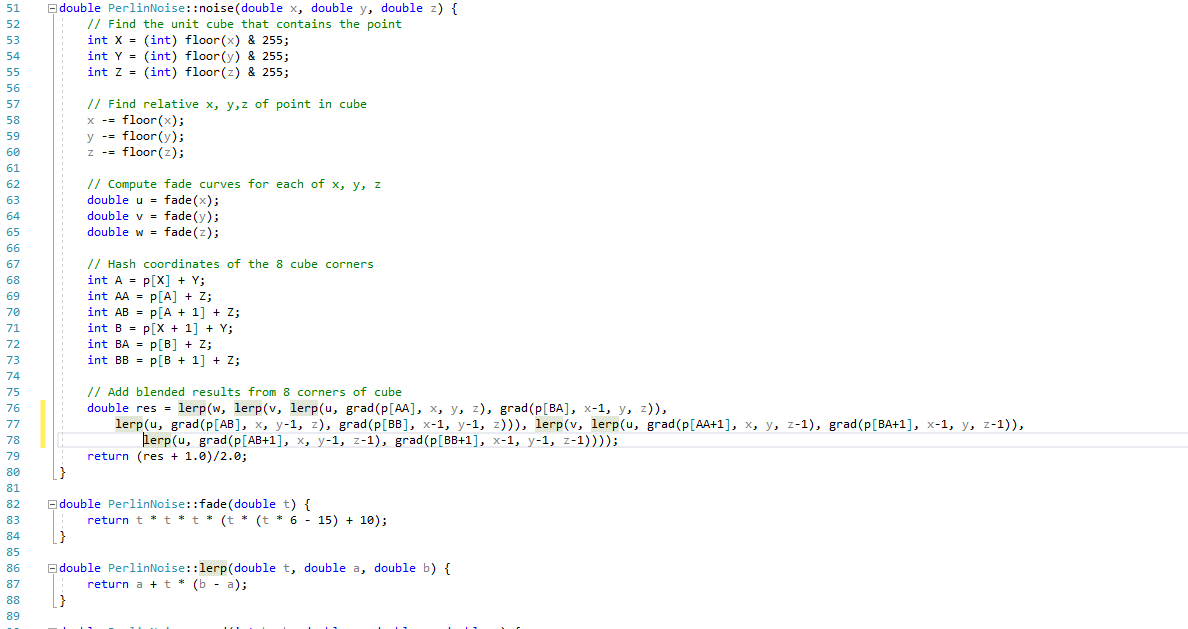
\includegraphics[width=1.0\textwidth]{images/code.png}
	\caption{Perlin Noise Calculations}
\end{figure}
\vspace{5mm} 
\newline
The X,Y,Z calculate the grid cell co-ordinates that contain the point. The next step is to find the relative point of x,y,z by subtracting the floor of each value. From this point it the algorithm will calculate the weight of the interpolation needed by performing the fade function. at this point the 8 points of the cube must be hashed out, once this has been completed the weights of the interpolation are lerped together and the noise is exported. 
\section{Binomial Distribution }
During the creation of the application it was quickly discovered that truly random map generation would never work as it likely hood of the map being completely unusable and would not pass the evaluation algorithm. To surpass this problem binomial distribution was used.
\begin{figure}[h]
	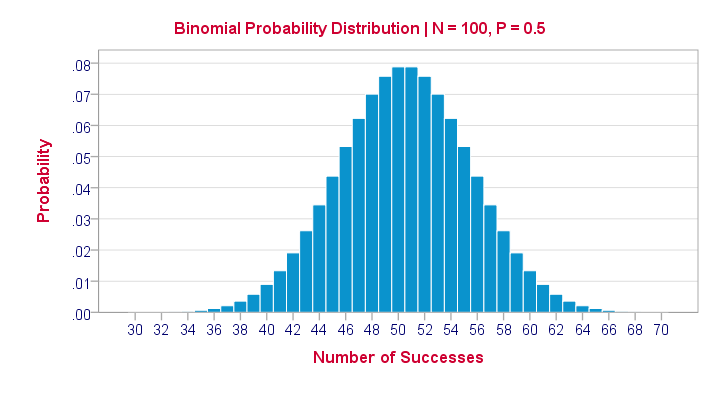
\includegraphics[width=1.0\textwidth]{images/binomial.png}
	\caption{A Binomial-Distribution Graph}
\end{figure}
\vspace{5mm} 
\newline
As shown above in figure 3.2, binomial distribution allows the probability of the central numbers to occur much more likely than the numbers that occur the further away from the median you travel. This was important to use within the project to greatly increase the chance of the map generator to producing a successful map. 
\vspace{5mm} 
\newline
\section{A* Modifications}
As described in section 2.5 A* algorithm was used in the map generation. This was to calculate the path that the payload travelled, however several modifications were made to the heuristic weight that was placed on each node. The reason for this was during the re-search into existing co-operative first person shooter maps\cite{Overwa}, a trend within each map was discovered each payload did not head along the shortest path. Instead it was down to the time which the payload took to reach each checkpoint. With the minimum time the payload took to complete each checkpoint being within five seconds of a minute. This changed the aim of the algorithm to not calculate the quickest route value but route which came closet to taking a minute to complete with the algorithm reflecting this change.
\vspace{5mm} 
\newline
\section{Height-mapping}
To easily visualize the maps that would be generated it was important to create a 3-D object from the noise generation. To do this a height-mapping would be used. Generating a mesh from a height map involves calculating the vertexs and indices of the  height-map depending on the shade of the texture. Once the vertexs and positions have been calculated,  the  mesh can be exported into an object loader to generate within the scene.  
\section{Evaluation Algorithm}
The first  stage of developing the evaluation algorithm was to state limits on equation, for this it was decided that the best result that the equation could produce was zero with the number getting larger the worse the map was. The equation was spilt into three parts each measuring a different aspect to the map. These were Size,Path and Balance once each was calculated the algorithm would add the values togethr to create a final map rating.   
\subsection{Size}
There were some difficulties when it came to designing the maps this was because the size of map is largely an arbitrary number which is highly depend on how quickly the player can cross the map. This lead the formula to be adapted from the physics formula: distance equals velocity multiplied by time. The final formula that was used was:  
\begin{equation}
\frac{(E(t)  - \frac{d}{v_c}))^2}{k}
\end{equation} 
Where  \(E(t) =\) the ideal time taken to complete the map which in this case was 60 seconds.
 \(\frac{d}{v_c}  =\) distance divided by time, this was calculated by applying Pythagoras theorem to the square to calculate the hypotenuse which equalled the distance and the velocity which equalled the players speed. If \((E(t)  - \frac{d}{v_c}) =\) was a negative this would shown the map was too big, while a positive number would relay a map that was too small. The equation was then squared to remove the negative and create the number that could be added to the final result. \(k \) became a constant that the user could choose to control the result by whichever aspect was more important to the user,for this project the constant was valued at 50;
\subsection{Path}
The path algorithm uses the exact same formula as the size formula however the values change slightly as the player's velocity is no longer evaluated and in their place is the payload that would be escorted's velocity. Also \(E(t) \) has changed to better reflect the speed of the payload which moves much slower than the player. this is represented by a \(_p \) character. Similarly to size equation a negative value lets the user know that the payload's path is too long but this is removed in the final equation. The constant for the path also rated at 50 as it was valued at a similar importance to the size of the map.  
\subsection{Balance}
The balance equation was far more complicated than the other aspects of the equation as it is difficult to quantify what a balanced map is. To represent this several objects were spawned into the map including buildings and health packs and their value calculated.
\begin{equation}
\frac{(\sum(\frac{o_a  w}{d}) - \sum(\frac{o_d w}{d})) ^2}{k_3} 
\end{equation}
In this equation \(o\) represents the objects of impact in the scene. These are split between where or not they spawn on the attacking (\(o_a\)) or defending(\(o_d\)) side of the map with at this point they are multiplied by the heuristic weight (\(w\)). This is calculated by how important the object is to game, ie health packs would have a much higher weight than a barrier. This value is then divided by distance(\(d\)) away from spawn of each team and added together with all other objects that exist. This value is also squared to remove the negative that could exist if the the defending team has an unfair advantage. In this instance the third constant was much lower than the other constants at 25 as fairness was concluded to be the most important factor of those being tested.
\subsection{Final Algorithm}
Once these three equation were combined they resulted in the final evaluation algorithm being equal to:  
\begin{equation}
\frac{(E(t_c)  - \frac{d_c}{v_c}))^2}{k_1} + \frac{(E(t_p)  - \frac{d_p}{v_p}))^2}{k_2} + \frac{(\sum(\frac{o_a  w}{d}) - \sum(\frac{o_d w}{d})) ^2}{k_3} 
\end{equation} 
This equation was then applied to the maps that were generated.
\section{Survey}
The survey was created following the guidelines discussed in SL McLafferty's book; Key methods in geography\cite{Geog}. While this might not be considered relevant to computer graphics it does state very useful guidelines to follow when creating a survey including:
\begin{itemize}
\item Keep questions simple.
\item Remove jargon.
\item Avoid long and complex questions.
\item Avoid biased and emotionally charged questions.
\end{itemize}
Using these guidelines a survey was created whit 6 questions that involved participants looking at a series of maps and answering questions based on their own background in playing co-operative fist person shooters. Once enough survey were to be filled out the results would be aggregated.    
%IMPLEMENTATION
\chapter{Implementation}
This section contains an in depth description of both the creation of the evaluation algorithm and the implementation of the procedurally generated co-operative first person shooter map. We will present the thematic choices that were made to optimize the successfulness of the map generation and the graphical choices such as height mapping that were made to easily visualize the map that was generated. To ensure the successfulness of both of the deliverables a survey was created that would allow the algorithm to be tested against users.
\vspace{5mm} 
\newline
\section{Programming Environment}
The applications were developed using Visual Studio 2017 Ultimate (Microsoft
2017) with the algorithm and application being written in C++. The graphics framework that was used was a combination of OpenGl and GLM \cite{OpenGL}. This allowed easy graphic manipulation which was important as it allowed more time to be spent on other aspects of the project.Through adding a header file that was imported from Github that already contained the Perlin noise algorithm within it, this helped with the exporting of image files that made it possible to easily view the terrain that had been generated. The survey was created using Microsoft Word to simplify the editing process for the users.  Version control was used during this project though GitHub which allowed easy access to the dissertation from anywhere.
\vspace{5mm} 
\newline
\section{Map Representation}
As outlined in section 3.4 the terrain of the map would be mapped out using height mapping, however each node of the path, building and other map features had to be represented in the scene as well. To do this each object was represented by a cubiod mesh in the scene with its own texture to be able to differentiate between them. As it was not possible to show participants in the survey the 3-D model another way to represent the map had to be devised.
\begin{figure}[h]
	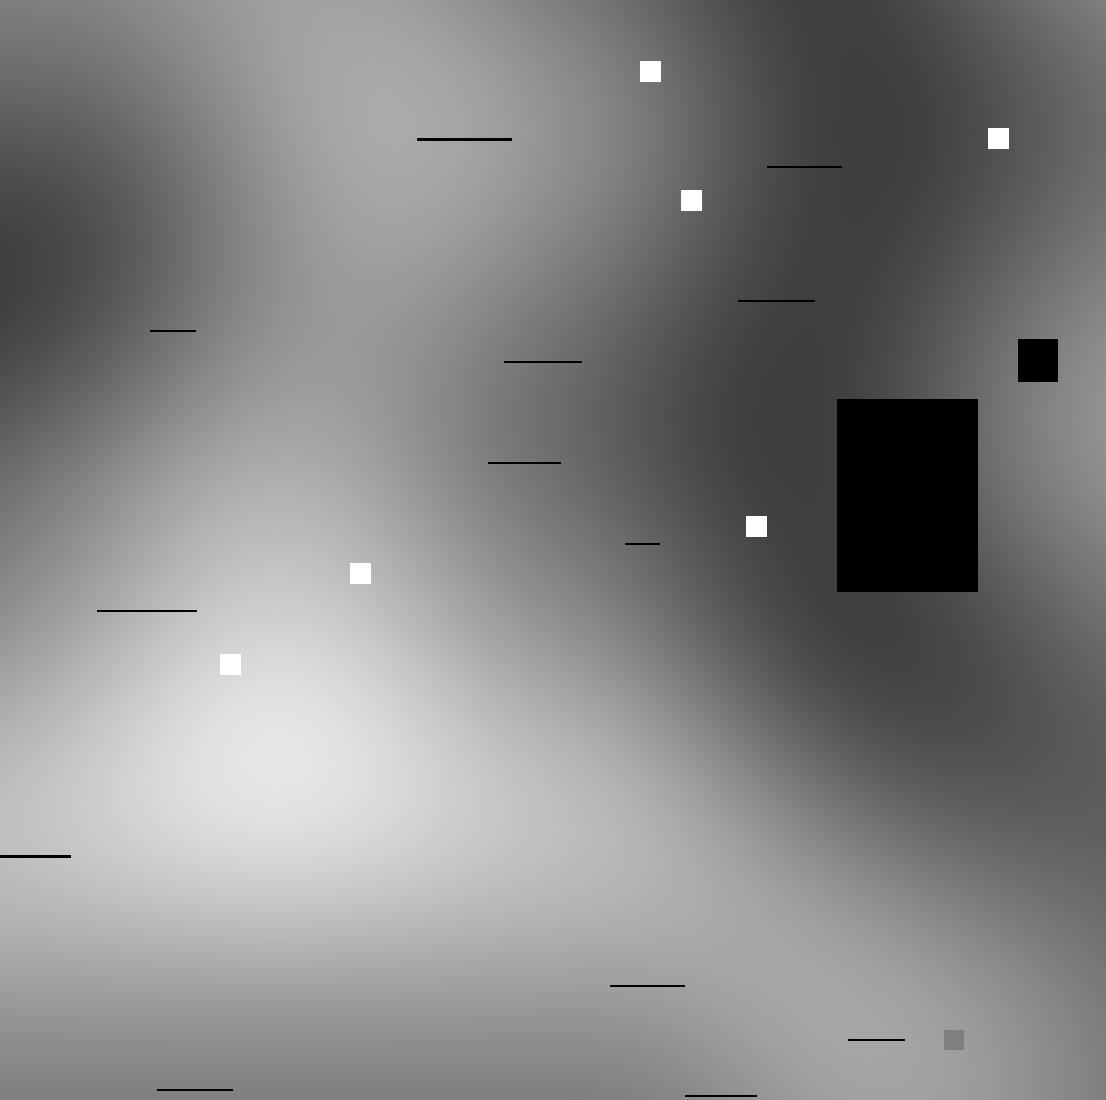
\includegraphics[width=\linewidth]{images/4.png}
	\caption{One of the generated map presented in the survey}
\end{figure}
\vspace{5mm} 
\newline 
 As shown in the figure above, this was the way the maps were shown to participants in the survey. They were also shown the key which explained that white nodes were the path of the payloads path, grey square were health packs and black square were buildings and objects. Participants were also told that the attacking team spawned at the top right corner, while the defending team spawned on the opposite bottom left corner.
\section{Thematics}
To provide some variety between the maps, A system was designed that would apply a theme to each map that was generated that would allow different play styles to occur and each map theme would differ in the chance of different buildings to spawn. The four different buildings that could occur were; Skyscrapers, Houses, Cars and Barriers. The theme of the map also affected other parts of the map such as the spawning location of health packs which could spawn within a building changing the importance of that building by a large amount. The spawn rates are as follows: 
\vspace{5mm} 
\newline 
\begin{tabular}{ |p{3cm}||p{2cm}|p{2cm}|p{2cm}|p{2cm}|  }
	\hline
	Theme& Skyscraper &Houses&Cars & Barriers\\
	\hline
	City   & 80\%    &0\% &   15\% & 5\%\\
	Desert & 0\%    &20\% &   15\% & 65\%\\
	Village &0\%    &50\% &   40\% & 10\%\\
	Seaside  &0\%    &50\% &   20\% &30\%\\
	\hline
\end{tabular} 
\vspace{5mm} 
\newline
The next sections detail other differences between the themes and the type of play style it attempts to replicate. 
\subsection{Types of Theme}
While the theme of the map does not affect two parts of the evaluation algorithm it is the main contributor to the third part of the calculation which during these tests was deemed to be the most important of the evaluation algorithm with the location of buildings and health packs making up a large part of the algorithm, each theme balances the map in their own way; The City cause a lot of close combat fighting with skyscrapers blocking off the many escape routes. This is nearly the opposite of Desert which offers wide open planes with cover being very difficult to find in certain parts of the map. The other two  themes are the average between the two other themes which allow a balance to be struck between the two extremes. 
%EVALUATION
\chapter{Results}
Three maps from the generated to be evaluated by both participants in the survey and the evaluation algorithm detailed in section 3.5
\section {Map 1}
The first map that was tested had a desert theme however unlike most desert maps that can be generated this map contined a large amount of houses that could be used as cover for either team.  
\begin{figure}[H]
	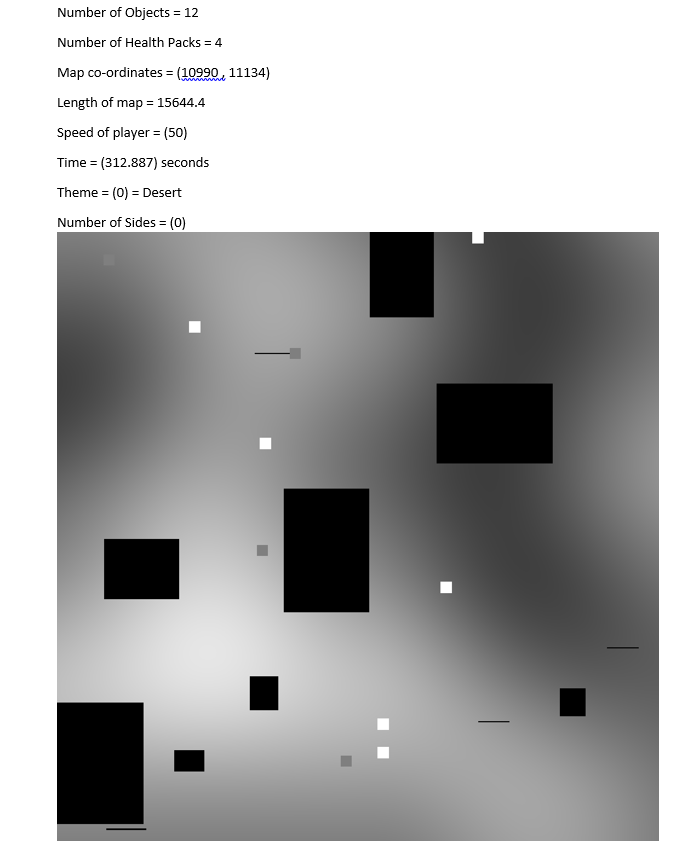
\includegraphics[width=0.7\textwidth]{images/map1.png}
	\caption{The First Map Presented as the Survey}
\end{figure}
\subsection{Survey Result}
\subsubsection{Map Size}
\begin{figure}[H]
	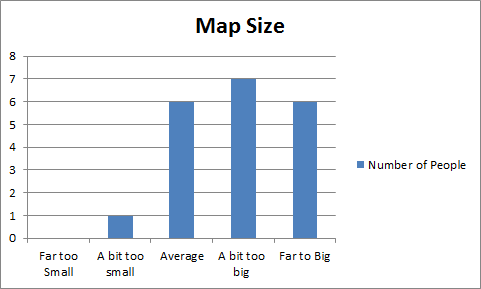
\includegraphics[width=1.0\textwidth]{images/Size1.png}
	\caption{Survey Data on the First Map Size}
\end{figure}
As shown in the graph above the map was considered to be larger than it needed to be. 
\subsubsection{Route}
\begin{figure}[H]
	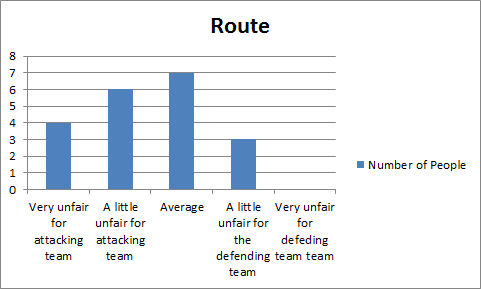
\includegraphics[width=1.0\textwidth]{images/Route1.png}
	\caption{Survey Data on First Map Route}
\end{figure}
As shown in the graph above the map was considered to slightly biased towards the attacking team.
\subsubsection{Fairness}
\begin{figure}[H]
	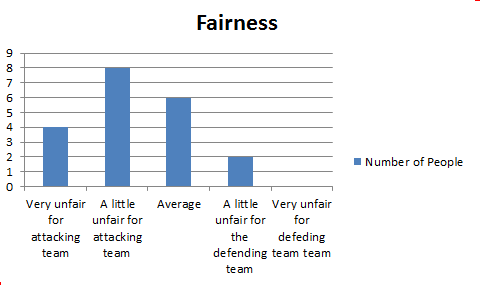
\includegraphics[width=1.0\textwidth]{images/Fair1.png}
	\caption{Survey Data on First Map Balance}
\end{figure}
Similarly to the previous survey it was considered slightly biased towards the attacking team.
\subsection{Evaluation Algorithm Result}
\begin{figure}[H]
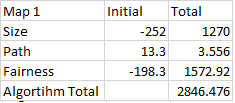
\includegraphics[width=0.5\textwidth]{images/algorithm.png}
\caption{The Evaluation Algorthm Rating the First Map }
\end{figure}
The output of the evaluation algorithm states that map is considered to be far too big to be a competitive map however it also states that the path is nearly perfect with the lowest score of the three variables however the fairness value is probably too high stating that the attacking team has an too great an unfair advantage to consider this a successful generation.
\section {Map 2}
\begin{figure}[H]
	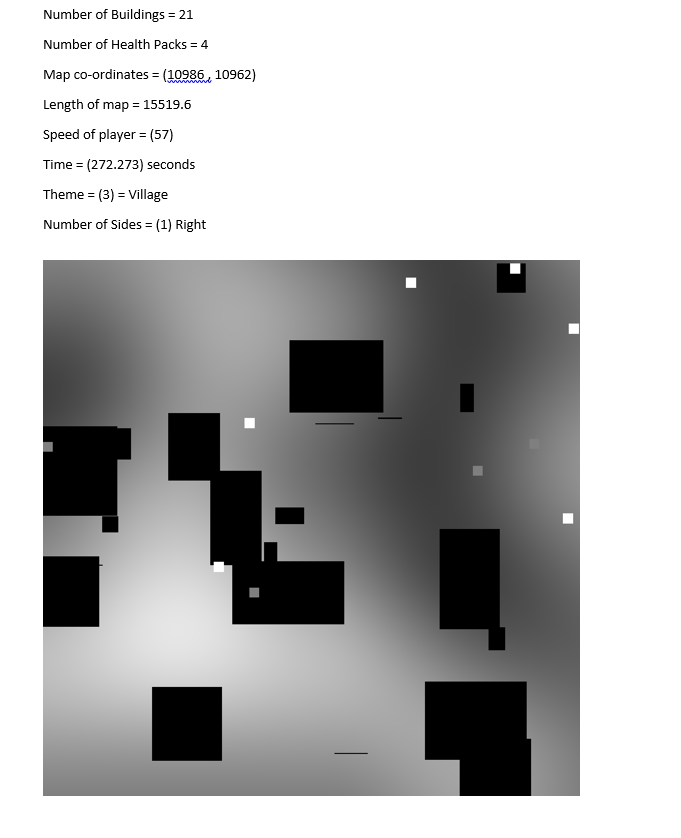
\includegraphics[width=1.0\textwidth]{images/map2.png}
	\caption{Nosie of the Second Map}
\end{figure}
The second  map is set as the village theme this caused more houses to be able to spawn in. Also in this map several health packs spawn within houses, if this occured in a real map players would fight much closer to these rooms as they provide cover as well as health. Therefore the heuristic weight of these health packs have been adjusted accordingly. 
\subsection{Survey Result}
\subsubsection{Map Size}
\begin{figure}[H]
	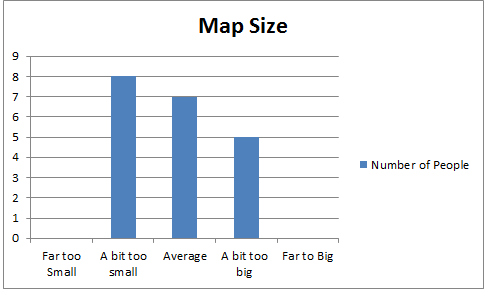
\includegraphics[width=1.0\textwidth]{images/Size2.png}
	\caption{Survey Data on the Second Map's Size}
\end{figure}
Within this figure the size of the map seems to be very close to being a good size with none of the surveyed participants stating that the map was too big or too small.
\subsubsection{Route}
\begin{figure}[H]
	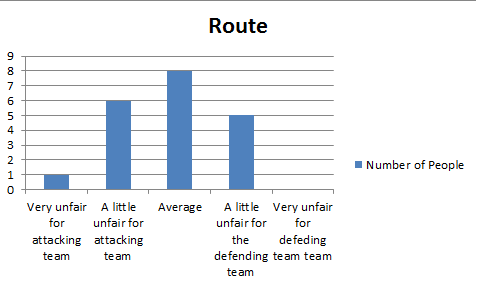
\includegraphics[width=1.0\textwidth]{images/Route2.png}
	\caption{Survey Data on the Second Map's Route}
\end{figure}

\subsubsection{Fairness}
\begin{figure}[H]
	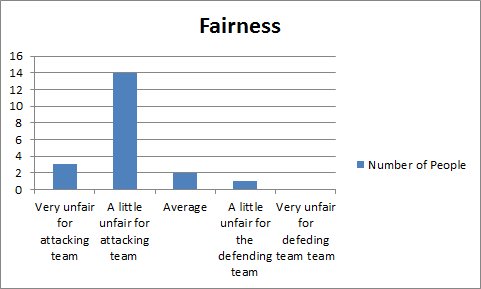
\includegraphics[width=1.0\textwidth]{images/Fair2.png}
	\caption{Survey Data on the Second Map's Fairness}
\end{figure}
\subsection{Evaluation Algorithm Result}
\begin{figure}[H]
	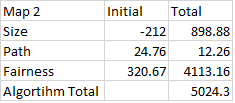
\includegraphics[width=0.5\textwidth]{images/a.png}
	\caption{The Evaluation Algorthm Rating of the Second Map}
\end{figure}
The evaluation of the map is given a very high rating this is largely because of how unbalanced the map is, while the map has equal health packs on either side both of the defending exist within cover while the attackers health packs exist very close together in the open which is not ideal for the attackers. Similarly to the first map the map is far too large to properly be considered to be a success however the path is very good on this map taking nearly exactly the right time to complete the map. 
\section {Map 3}
The third map was also a desert theme however unlike the first map this map contains far more barriers and lacks the amount of houses that existed in the first one. The only health pack that exists down in the bottom right corner nearly equal distance between the two spawns. 
\begin{figure}[H]
	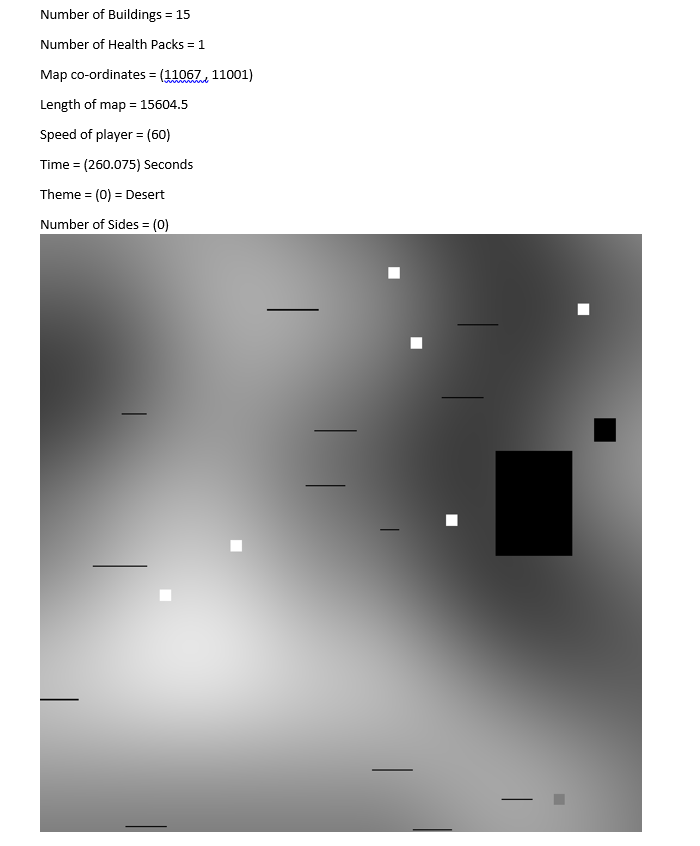
\includegraphics[width=1.0\textwidth]{images/map3.png}
	\caption{Survey Data on Map Size}
\end{figure}
\subsubsection{Map Size}
\begin{figure}[H]
	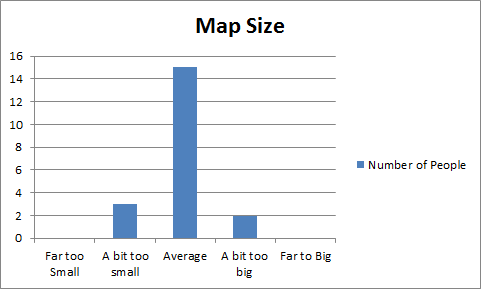
\includegraphics[width=1.0\textwidth]{images/Size3.png}
	\caption{Survey Data on the Third Map's Size}
\end{figure}
\subsubsection{Route}
\begin{figure}[H]
	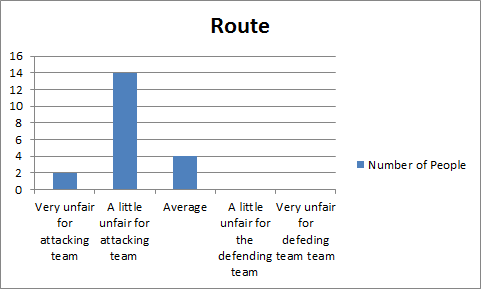
\includegraphics[width=1.0\textwidth]{images/Route3.png}
	\caption{Survey Data on the Third Map's Route}
\end{figure}
\subsubsection{Fairness}
\begin{figure}[H]
	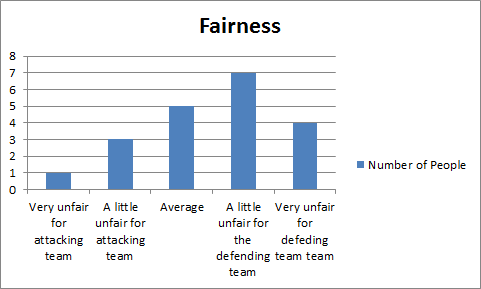
\includegraphics[width=1.0\textwidth]{images/Fair3.png}
	\caption{Survey Data on the Third Map's Fairness}
\end{figure}
\subsection{Evaluation Algorithm Result}
\begin{figure}[H]
	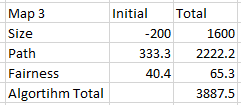
\includegraphics[width=0.5\textwidth]{images/alg.png}
	\caption{The Evaluation Algorthm Rating the Third Map }
\end{figure}
While the might be the worst map for paths and distance the balance of this map is nearly the ideal value. This is because as stated above the only health pack exists nearly equal between the two spawns however while it is slightly closer to the defending spawn the attackers spawn offsets this by having two buildings within close proximity to the spawn allowing for the most balanced map that was tested to occur.
%CONCLUSION
\chapter{Conclusion}
\section{Discussion of Results}
From the set of results that are extrapolated from the first map, there is several positives to be taken from this data. Firstly the algorithm and the survey agree that the map is far too large to be considered a successful map however it is much more important that the equation agrees with the survey rather than the algorithm agree with the map generator. In the case of the route from map 1 this was the best value that was received from the test with the survey and the algorithm agreeing that the path was close to being the ideal value. This was very uplifting to here as the map generation slightly struggles to create consistently good maps.
\vspace{5mm} 
\newline 
For the second set of results the biggest inconsistency occurred here with the size of the map being similar to map 1 the survey adjudged it to be an adequate size however the algorithm judged it too be too big again and it is probably the correct assumption to make that the algorithm is correct and maybe it should be considered to conduct more surveys to be able to be sure.
\vspace{5mm} 
\newline 
Map 3 was the most successful of all the maps in regards to fairness which during this test was deemed to be the most important factor being tested therefore it is not unreasonable to say that this was the most successful map hands down, this combined with the fact that none of the maps correctly generated the size and this must be changed at a future date to generate the correct values, however this is a simple enough fix and would greatly improve the procedural map generator. 
\vspace{5mm} 
\newline   
From the results that have been gathered it would be easy to say that while the evaluation algorithm is working as intended and its counter-part the procedural map generator was not working as well as it could be, and while this is most likely the case it is important to note that the map generator stared off by producing maps that were rated at over 15,000 which now to be producing maps that go under the 3,000 is a big achievement and with more time could be able to produce much lower rated maps. 
\vspace{5mm} 
\newline 
\section{Fulfilment of Aims and Objectives}
 This project has resulted in successful implementation of a procedural map generator that adheres to the aims and objectives that were set during the initial planning phase. The tests that were designed tested each map the way that was initially planned to collect three metrics size, path and fairness.  
 \vspace{5mm} 
\newline
The results collected from these tests allowed us to gain an understanding of how the evaluation algorithm performed and behaved when faced with different types of obstacles allowing us to to edit and change the formula easily and be able to correctly judge how well the procedural map generation was performing, this in turn lead to a much more successful project than  was expected after the procedural map generator continually under-performed. 

\section{Future Work}
The procedural map generator could benefit greatly from several optimizations, firstly it could successfully be integrated with a parallelization techniques such as OpenMP or CUDA to speed up the time taken to generate the Perlin's noise or A* algorithm which both take a large time to create. 
\vspace{5mm} 
\newline
Another improvement that could be made could be to implement individual models for the objects that reside in the scene because of the lack of knowledge for creating these models in MAYA or blender, however this could add a great extra aspect to the 3-D scene that was created.
\vspace{5mm} 
\newline
The evaluation algorithm could also benefit from several optimizations, while the algorithm was purposely created to be open ended, different parts of the map could be tested such as the choke points.   
\section{Critical Assessment of Project} 
I believe that the evaluation algorithm works better than I had ever expected however I was extremely disappointed with the performance of the map generation device as this caused countless problems along the way, however I still believe that I chose all the correct techniques when creating the system and the reason for the underperformance was poor planning not allowing for enough time just in case errors occurred.  This was the main regret from all  this entire project was not enough planning and this will have affected the quality of my dissertation.
\newpage

\bibliographystyle{plain}
\bibliography{bibfile}

\newpage
\begin{appendices}
\section*{A Initial Project Overview Document}
\subsection*{Title of Project}
Evaluation of Procedural generation of Escort Maps
\subsection*{Overview of Project Content and Milestones}
Team based shooters are some of the most popular games currently with Overwatch being one of the biggest of these games. A game mode of team based shooters is Escort missions where the attacking team must push a payload to a certain distance while the defending team tries to stop them.
\vspace{5mm} 
\newline
The aim of this project is to design an algorithm that rates the maps escort missions are played on and design an application that procedurally generates a map that adheres to the algorithm. 
\vspace{5mm} 
\newline
Milestones:
\newline
Decide on what makes a successful escort mission map by looking at pre-existing maps.
\newline
Design an algorithm that uses the information from the milestone before. 
\newline
Create a system that procedurally generates escort mission maps.
\newline
Use the algorithm to improve the system that was built. 
\subsection*{The Main Deliverable(s):}
An algorithm that can evaluate escort mission maps.
\newline
An application that can procedurally generate a map 
\newline
The final dissertation of the findings from this project 
\subsection*{The Target Audience for the Deliverable(s):}
The main audience for this project would be companies or developers who are interested in creating a game that uses escort missions as a game mode and could use the algorithm to improve the maps they created.
\subsection*{The Work to be Undertaken:}
The work to be undertaken will be to create an algorithm that can define whether a map is good nor not. This will involve testing several published maps and reading papers on this subject. From there the algorithm will start to be created taking into account map size, the payloads path and balancing for the attacking and defending team. This algorithm will then be implemented in a c++ program to create maps and discard the unsuccessful maps. Basic art assets will also be produced for the map i.e. the payload and building blocks. The findings will then recorded in a paper and on a poster.
\subsection*{Additional Information / Knowledge Required:}
Extra information will be needed in several fields such as researching more existing maps to get a better idea of these maps have in common. More research will also be done in procedural generation.
\subsection*{Information Sources that Provide a Context for the Project:}
Adaptively Challenges in Games
\newline
What makes a game good?
\newline
Procedurally generating cities 
Yoav I. H.Parish, Pascal Müller
\subsection*{The Importance of the Project:}
Why this project is important is to be used by companies and individuals creating maps for team based shooters to be able to rate their map before the player testing phase and to streamline the testing phase as the user would already have an idea if the map would be successful or not.
\subsection*{The Key Challenge(s) to be Overcome:}
A major challenge in this project will be learning procedural generation as I have never used procedural before another issue will be defining what a good map is, as this up to a point is completely subjective and while one person may enjoy a map someone else might not.
\vspace{5mm} 
\newline
\section*{B Week 9 Interim Report}
Aims and Objectives:
There are two main aims of the project, the first is to create, implement and evaluate an algorithm that assesses escort mission maps once this has been complete, the next aim is to plan and develop a piece of software that can successfully follow the algorithm produced. The objectives below have been selected in order to accomplish these aims.
Research relevant topics and papers.
Create or use an existing framework that can be used to develop the map.
Design an algorithm taking into account size, path of the payload and fairness.
Develop a programme that can procedurally generate escort mission maps.

\subsection*{Progress:}
The first part of this project that was decided on was the plan of work. It was decided that the algorithm and the scene would be developed simultaneously because this would allow it to be easier to edit the program if changes were made to the algorithm at a later date. Once this had been complete it was time to plan out how the algorithm would work. The idea for the algorithm would be that 0 would be the best possible map the greater the number the worse the map would be. Work then began on the first part of the algorithm which was how to calculate the ideal size of the map. While size is difficult to calculate as there is no standardized measurements however what can be measured is time so in several pre-existing maps, the time taken to walk from point A to B was measured to see if any patterns could be noticed. Every map took 1 minute plus or minus 10\% to complete this allowed an ideal time to be calculated and could be inserted into the formula that had been already decided on.
\newline
\((E(t)-(d/v)^2)/k\)
\newline
E(t) = ideal time 
d is distance of plane
v is speed of player 
k is a constant that will be dependent on how important size of the map is
Above is the size formula that has been decided on. Once this was complete it was time to decide on which framework would be worked on. The decision was decided to work inside. It was decided to work with the graphics framework. The reasoning for this was mainly down to personal preference as it was a framework that had been used before and was considered robust enough to handle the work that was needed. 
Work then began with the graphics frame work a simple program was set up to create a randomly generated plane that would change its size every time it ran. After this work began on generating then path that the escorting object would follow began. 
Research began into existing pathfinding algorithms and the most common pathfinding algorithm that was found was A* this could be used with a grid that was rendered on top of the plane that had already been created. The A* algorithm also needed nodes to create a path through it was decided that the nodes would be procedurally generated using a procedural generation algorithm found online called Auburn’s fast noise this has a variety of different procedural generation so the preferable generations would be call or value as these offer an obvious distinction between nodes and blank space. 
Implementation of these techniques was began.
Some future planning that has been done is planning the pipeline of how that map will be created. It would go through several stages like so
Spawn a plane of varying size.
Spawn start and end points for the payload.
Procedurally generate nodes for the path of the object.
Use the A* algorithm to plot the route.
Smooth the path drawn at stage 4.
Procedurally generate a level above and below the plane.
Attach walkways and connectors too the three levels.
Spawn in obstacles and buildings.
This is also similar to how the plan to develop this application works.   

\subsection*{Plan:}
The plan that was decided on was too create the algorithm and application simultaneously so that the application stays close to the algorithm. This means that once it has been decided on how certain part of the algorithm works that part of the system which it tests will be coded. No dates where attached these tasks accept for general guidelines Therefore this is how the plan/task list will look:
Research how the algorithm works 
Create algorithm for the size of map
Re-search Procedural generation and which framework to use
Create basic plane with restrictions that follow the algorithm
Create algorithm for start and end point.
Render in start and end points
Create rating system for the path of the payload
Add in the path between start and end point 
Create an algorithm that rates the balance of the map 
Add in dead-zones and chokepoints into the map. 

\subsection*{Evaluation:}
The way that this project will be evaluated is through two major ways the first being that the maps will be evaluated will be through users testing the maps that are generated by the programme the users will all have experience with playing escort mission maps and will fill out a survey after looking through the maps. The survey will be closed questions with questions such as: What do you think of the size of the map? Would you enjoy playing this map? If the users rate the map similar to the algorithm then it would be judged to be a successful. From this point if the algorithm is classed as successful the procedurally generated maps will use the algorithm to generate better maps. The other way that the project will be evaluated is through testing pre-existing maps through the algorithm that has been created. While this is not the main way of testing the project it will allow a final evaluation for the project and add consistency to the results that were produced.    

\section*{C Diary Sheets}

\section*{D Consent Forms and Questionaires}

\end{appendices}

\end{document}
